\documentclass[journal,12pt,twocolumn]{IEEEtran}

\usepackage{setspace}
\usepackage{gensymb}

\singlespacing


\usepackage[cmex10]{amsmath}

\usepackage{amsthm}

\usepackage{mathrsfs}
\usepackage{txfonts}
\usepackage{stfloats}
\usepackage{bm}
\usepackage{cite}
\usepackage{cases}
\usepackage{subfig}

\usepackage{longtable}
\usepackage{multirow}

\usepackage{enumitem}
\usepackage{mathtools}
%\usepackage{steinmetz}
\usepackage{tikz}
\usepackage{circuitikz}
\usepackage{verbatim}
%\usepackage{tfrupee}
\usepackage[breaklinks=true]{hyperref}

\usepackage{tkz-euclide}

\usetikzlibrary{calc,math}
\usepackage{listings}
    \usepackage{color}                                            %%
    \usepackage{array}                                            %%
    \usepackage{longtable}                                        %%
    \usepackage{calc}                                             %%
    \usepackage{multirow}                                         %%
    \usepackage{hhline}                                           %%
    \usepackage{ifthen}                                           %%
    \usepackage{lscape}     
\usepackage{multicol}
\usepackage{chngcntr}

\DeclareMathOperator*{\Res}{Res}

\renewcommand\thesection{\arabic{section}}
\renewcommand\thesubsection{\thesection.\arabic{subsection}}
\renewcommand\thesubsubsection{\thesubsection.\arabic{subsubsection}}

\renewcommand\thesectiondis{\arabic{section}}
\renewcommand\thesubsectiondis{\thesectiondis.\arabic{subsection}}
\renewcommand\thesubsubsectiondis{\thesubsectiondis.\arabic{subsubsection}}


\hyphenation{op-tical net-works semi-conduc-tor}
\def\inputGnumericTable{}                                 %%

\lstset{
%language=C,
frame=single, 
breaklines=true,
columns=fullflexible
}
\begin{document}


\newtheorem{theorem}{Theorem}[section]
\newtheorem{problem}{Problem}
\newtheorem{proposition}{Proposition}[section]
\newtheorem{lemma}{Lemma}[section]
\newtheorem{corollary}[theorem]{Corollary}
\newtheorem{example}{Example}[section]
\newtheorem{definition}[problem]{Definition}

\newcommand{\BEQA}{\begin{eqnarray}}
\newcommand{\EEQA}{\end{eqnarray}}
\newcommand{\define}{\stackrel{\triangle}{=}}
\bibliographystyle{IEEEtran}
\providecommand{\mbf}{\mathbf}
\providecommand{\pr}[1]{\ensuremath{\Pr\left(#1\right)}}
\providecommand{\qfunc}[1]{\ensuremath{Q\left(#1\right)}}
\providecommand{\sbrak}[1]{\ensuremath{{}\left[#1\right]}}
\providecommand{\lsbrak}[1]{\ensuremath{{}\left[#1\right.}}
\providecommand{\rsbrak}[1]{\ensuremath{{}\left.#1\right]}}
\providecommand{\brak}[1]{\ensuremath{\left(#1\right)}}
\providecommand{\lbrak}[1]{\ensuremath{\left(#1\right.}}
\providecommand{\rbrak}[1]{\ensuremath{\left.#1\right)}}
\providecommand{\cbrak}[1]{\ensuremath{\left\{#1\right\}}}
\providecommand{\lcbrak}[1]{\ensuremath{\left\{#1\right.}}
\providecommand{\rcbrak}[1]{\ensuremath{\left.#1\right\}}}
\theoremstyle{remark}
\newtheorem{rem}{Remark}
\newcommand{\sgn}{\mathop{\mathrm{sgn}}}
\providecommand{\abs}[1]{\left\vert#1\right\vert}
\providecommand{\res}[1]{\Res\displaylimits_{#1}} 
\providecommand{\norm}[1]{\left\lVert#1\right\rVert}
%\providecommand{\norm}[1]{\lVert#1\rVert}
\providecommand{\mtx}[1]{\mathbf{#1}}
\providecommand{\mean}[1]{E\left[ #1 \right]}
\providecommand{\fourier}{\overset{\mathcal{F}}{ \rightleftharpoons}}
%\providecommand{\hilbert}{\overset{\mathcal{H}}{ \rightleftharpoons}}
\providecommand{\system}{\overset{\mathcal{H}}{ \longleftrightarrow}}
	%\newcommand{\solution}[2]{\textbf{Solution:}{#1}}
\newcommand{\solution}{\noindent \textbf{Solution: }}
\newcommand{\cosec}{\,\text{cosec}\,}
\providecommand{\dec}[2]{\ensuremath{\overset{#1}{\underset{#2}{\gtrless}}}}
\newcommand{\myvec}[1]{\ensuremath{\begin{pmatrix}#1\end{pmatrix}}}
\newcommand{\mydet}[1]{\ensuremath{\begin{vmatrix}#1\end{vmatrix}}}
\numberwithin{equation}{subsection}
\makeatletter
\@addtoreset{figure}{problem}
\makeatother
\let\StandardTheFigure\thefigure
\let\vec\mathbf
\renewcommand{\thefigure}{\theproblem}
\def\putbox#1#2#3{\makebox[0in][l]{\makebox[#1][l]{}\raisebox{\baselineskip}[0in][0in]{\raisebox{#2}[0in][0in]{#3}}}}
     \def\rightbox#1{\makebox[0in][r]{#1}}
     \def\centbox#1{\makebox[0in]{#1}}
     \def\topbox#1{\raisebox{-\baselineskip}[0in][0in]{#1}}
     \def\midbox#1{\raisebox{-0.5\baselineskip}[0in][0in]{#1}}
\vspace{3cm}
\title{EE5609 Assignment 5}
\author{SHANTANU YADAV, EE20MTECH12001 }
\maketitle
\newpage
\bigskip
\renewcommand{\thefigure}{\theenumi}
\renewcommand{\thetable}{\theenumi}

The python solution code is available at
\begin{lstlisting}
https://github.com/Shantanu2508/Matrix_Theory/blob/master/Assignment_5/assignment5.py
\end{lstlisting}

\section{Problem}
Find the value of $k$ so that the following equation may represent pairs of straight lines.
\begin{align*}
	12x^2 + xy -6y^2 -29x +8y +k =0 
\end{align*}
Also, find the equations of the lines.

\section{Explanation}
The general equation of second degree is given by
\begin{align}
	ax^2 + 2bxy +cy^2 +2dx +2ey +f =0            \label{eq1}
\end{align}
and can be expressed as
\begin{align}
	\vec{x}^{T}\vec{Vx} + 2\vec{u}^{T}\vec{x} + f=0   \label{eq2}
\end{align}
where
\begin{align}
	\vec{V}=\vec{V}^T=\myvec{a & b \\ b & c}   \label{eq3}  \\
	\vec{u}^T=\myvec{d &  e}            \label{eq4}
\end{align}
(\ref{eq1}) represents a pair of straight lines if
\begin{align}
	\mydet{\vec{V} & \vec{u} \\ \vec{u}^T & f} = 0     \label{eq5} 
\end{align}
The lines intercept if
\begin{align}
	\mydet{\vec{V}} < 0
\end{align}

\section{Solution}
From (\ref{eq3}) and (\ref{eq4})
\begin{align}
	\vec{V}=\vec{V}^T &= \myvec{12 & \frac{1}{2} \\ \frac{1}{2} & -6} \\
	\vec{u} &= \myvec{\frac{29}{2} \\ 4}
\end{align}
From (\ref{eq1}) and (\ref{eq5})
\begin{align}
	& \mydet{12 & \frac{1}{2} & -\frac{29}{2} \\ 
	       \frac{1}{2} & -6 & 4     \\
	       -\frac{29}{2} & 4 & k } = 0 \\  \nonumber \\
	 \implies \quad 12\mydet{-6 & 4 \\ 4 & k} &-\frac{1}{2}\mydet{\frac{1}{2} & 4 \\ 
	 				-\frac{29}{2} & k}
	-\frac{29}{2}\mydet{\frac{1}{2} & -6 \\ -\frac{29}{2} & 4} = 0 \\
	 \implies \quad & k =14
\end{align}
Since $ \vec{V} = \vec{V}^T $, there exists an orthogonal matrix $\vec{P}$ such that
\begin{align}
	\vec{P}\vec{V}\vec{P}^T = \vec{D} = diag\myvec{\lambda_1 & \lambda_2}
\end{align}
or equivalently 
\begin{align}
	\vec{V} = \vec{P}\vec{D}\vec{P}^T
\end{align}
Eigen vectors of real symmetric matrix $\vec{V}$ are orthogonal. The characteristic equation of $\vec{V}$ is obtained by evaluating the determinant
\begin{align}
	\mydet{\lambda\vec{I}-\vec{V}} = \mydet{\lambda-12 & -\frac{1}{2} \\ -\frac{1}{2} & \lambda +6} = 0 \\
	\implies \quad \lambda^2-6\lambda-\frac{289}{4}=0 \\
	\implies \quad \lambda_1=-\frac{483}{72},\lambda_2=\frac{865}{72}
\end{align}
The eigen vector $\vec{p}$ is defined as
\begin{align}
	\vec{V}\vec{p}=\lambda\vec{p} \\
	\implies (\lambda\vec{I} - \vec{V})\vec{p}=0
\end{align}
The orthogonal eigen-vector matrix
\begin{align}
	\vec{P}=\frac{1}{\norm{\vec{p}}}\myvec{\vec{p_1} & \vec{p_2}}
	=\myvec{\frac{24}{865} & \frac{-2596}{2597} \\  & \\ 
	-\frac{2596}{2597} & \frac{24}{865}} \\  \nonumber \\
	\vec{D}=\myvec{-\frac{433}{72} & 0 \\ & \\ 0 & \frac{865}{72}}
\end{align}
Let $\vec{x}=\vec{P}\vec{y} + \vec{c} $ with $\vec{c}=-\vec{V}^{-1}\vec{u}$. Substituting in \ref{eq2}
\begin{align}
	\vec{y}^T\vec{D}\vec{y}=\vec{u}^T\vec{V}^{-1}\vec{u}-f \\
	\implies \quad \vec{y}^T\vec{D}\vec{y}=0 \\
	\implies \quad \myvec{\pm\sqrt{\frac{\lambda_1}{\lambda_2}} & 1}\vec{y}=0   \label{eq6}
\end{align}
Substituting $\vec{y}=\vec{P}^T\vec{x} - \vec{P}^T\vec{c}$ in \ref{eq6} 
\begin{align}
	\implies \quad \myvec{\pm{\frac{1}{\sqrt{2}}} & 1}(\vec{\vec{P}^T\vec{x}-\vec{P}^T\vec{c}})=0 
\end{align}
The equations of lines are 
\begin{align}
	\myvec{\frac{49}{50} & \frac{37}{50}}\vec{x} = \frac{343}{200} \\
	\myvec{\frac{51}{50} & -\frac{34}{50}}\vec{x} = \frac{34}{50} 
\end{align}
\begin{figure}[!h]
	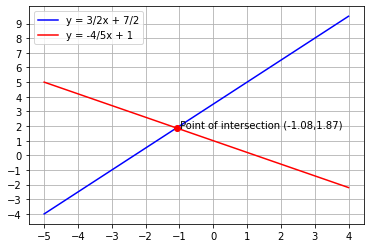
\includegraphics[width=\columnwidth]{lines.png}
	\caption{} \label{linefig1}
\end{figure}
\end{document}
